\documentclass{../zirkelblatt}

\usepackage{geometry}
\geometry{tmargin=0.5cm,bmargin=0.5cm,lmargin=1cm,rmargin=1cm}

\pagestyle{empty}

\begin{document}

\newcommand{\vorderseite}{
  \begin{minipage}[t][4cm][t]{8.5cm}
    \begin{center}
      \textsf{Die Kreiszahl~$\pi$, eine transzendente Zahl}
    \end{center}
    \vspace{-0.6em}
    \tiny
    \scalebox{1.12}{141 592 6535 897 932 3846 264 338 3279 502 884 1971 693 993 7510}

    \scalebox{1.12}{582 097 4944 592 307 8164 062 862 0899 862 803 4825 342 117 0679}

    \scalebox{1.12}{821 480 8651 328 230 6647 093 844 6095 505 822 3172 535 940 8128}

    \scalebox{1.12}{481 117 4502 841 027 0193 852 110 5559 644 622 9489 549 303 8196}

    \scalebox{1.12}{442 881 0975 665 933 4461 284 756 4823 378 678 3165 271 201 9091}

    \scalebox{1.12}{456 485 6692 346 034 8610 454 326 6482 133 936 0726 024 914 1273}

    \scalebox{1.12}{724 587 0066 063 155 8817 488 152 0920 962 829 2540 917 153 6436}

    \scalebox{1.12}{789 259 0360 011 330 5305 488 204 6652 138 414 6951 941 511 6094}

    \scalebox{1.12}{330 572 7036 575 959 1953 092 186 1173 819 326 1179 310 511 8548}

    \scalebox{1.12}{074 462 3799 627 495 6735 188 575 2724 891 227 9381 830 119 4912}

    \vfill
    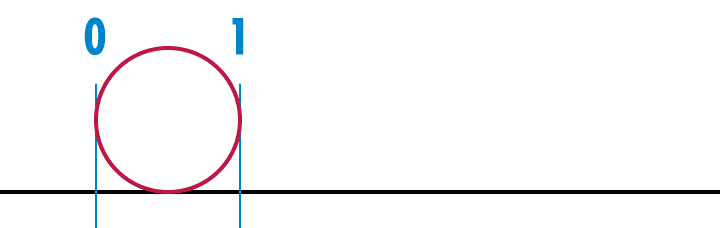
\includegraphics[scale=0.078]{pi-1}\hfill%
    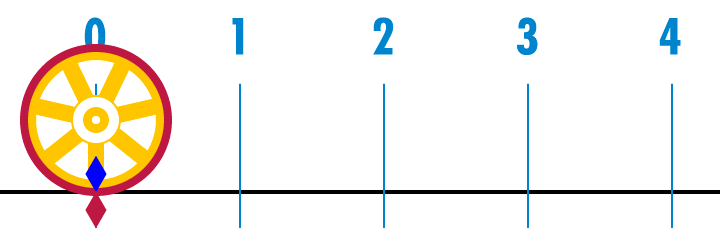
\includegraphics[scale=0.078]{pi-2}\hfill%
    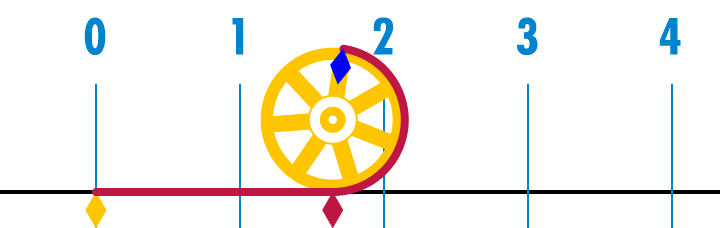
\includegraphics[scale=0.078]{pi-3}\hfill%
    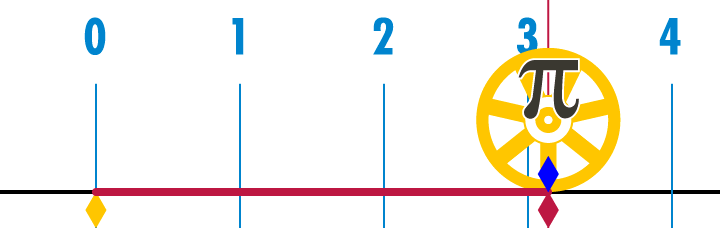
\includegraphics[scale=0.078]{pi-4}
  \end{minipage}
}

\newcommand{\rueckseite}{
  \begin{minipage}[t][4cm][t]{8.5cm}
    \phantom{A}
    \vspace{-0.3em}
    \tiny

    Die Kreiszahl~$\pi$ ist ungefähr 3: $\pi = 3{,}141\ldots$
    Eine gute \textbf{Näherung} ist $\pi \approx 22:7$, eine noch bessere ist~$\pi
    \approx 333:106$. Das liegt an der \textbf{Kettenbruchentwicklung}
    von~$\pi$.
    Das Symbol ist ein Buchstabe aus dem griechischen Alphabet und wird
    \textbf{Pi} ausgesprochen.
    Am 14. März feiern Fans den internationalen \textbf{$\pi$-Tag}.
    Bei Stelle~763 stehen \textbf{sechs Neuner} hintereinander.
    Der \textbf{Umfang} eines Kreises mit Radius~$r$ ist $2 \pi r$. Der
    \textbf{Flächeninhalt} ist~$\pi r^2$. Das \textbf{Volumen} einer Kugel
    mit Radius~$r$ ist~$\frac{4}{3} \pi r^3$.
    Die Zahl~$\pi$ ist \textbf{irrational}, lässt sich also nicht als Bruch
    zweier ganzer Zahlen schreiben. Außerdem ist sie sogar
    \textbf{transzendent}, also keine Lösung einer Polynomgleichung.
    \textbf{Offene Frage:} Kommen im Durchschnitt die zehn Ziffern in der
    Dezimalentwicklung von~$\pi$ gleich oft vor?
    \scalebox{0.7}{\begin{minipage}{1.42\textwidth}
    \vspace{-1.3em}
    \begin{align*}
      1 - \frac{1}{3} + \frac{1}{5} - \frac{1}{7} + \frac{1}{9} - \dots &= \frac{\pi}{4} &
      0 &= e^{i \pi} + 1 &
      \pi &= \int\limits_{-\infty}^\infty \frac{dx}{1+x^2} \\
      \frac21 \cdot \frac23 \cdot \frac43 \cdot \frac45 \cdot \frac65 \cdot
      \frac67 \cdot \frac87 \cdot \frac89 \cdot \dots &= \frac{\pi}2 &
      \chi(M) &= \frac{1}{2\pi} \int_M K \,dA &
      f(z) &= \frac{1}{2\pi i} \oint \frac{f(\zeta)}{\zeta - z} \,d\zeta
    \end{align*}\end{minipage}}
  \end{minipage}
}

\vorderseite\hfill\vorderseite
\vfill
\vorderseite\hfill\vorderseite
\vfill
\vorderseite\hfill\vorderseite
\vfill
\vorderseite\hfill\vorderseite
\vfill
\vorderseite\hfill\vorderseite

\newpage

\fontfamily{kurier}\selectfont

\rueckseite\hfill\rueckseite
\vfill
\rueckseite\hfill\rueckseite
\vfill
\rueckseite\hfill\rueckseite
\vfill
\rueckseite\hfill\rueckseite
\vfill
\rueckseite\hfill\rueckseite

\end{document}

983 367 3362 440 656 6430 860 213 9494 639 522 4737 190 702 1798
609 437 0277 053 921 7176 293 176 7523 846 748 1846 766 940 5132
000 568 1271 452 635 6082 778 577 1342 757 789 6091 736 371 7872
146 844 0901 224 953 4301 465 495 8537 105 079 2279 689 258 9235
420 199 5611 212 902 1960 864 034 4181 598 136 2977 477 130 9960
518 707 2113 499 999 9837 297 804 9951 059 731 7328 160 963 1859
502 445 9455 346 908 3026 425 223 0825 334 468 5035 261 931 1881
710 100 0313 783 875 2886 587 533 2083 814 206 1717 766 914 7303
598 253 4904 287 554 6873 115 956 2863 882 353 7875 937 519 5778
185 778 0532 171 226 8066 130 019 2787 661 119 5909 216 420 1989
380 952 5720 106 548 5863 278 865 9361 533 818 2796 823 030 1952
035 301 8529 689 957 7362 259 941 3891 249 721 7752 834 791 3151
557 485 7242 454 150 6959 508 295 3311 686 172 7855 889 075 0983
817 546 3746 493 931 9255 060 400 9277 016 711 3900 984 882 4012
858 361 6035 637 076 6010 471 018 1942 955 596 1989 467 678 3744
944 825 5379 774 726 8471 040 475 3464 620 804 6684 259 069 4912
933 136 7702 898 915 2104 752
